\documentclass{l3proj}

\begin{document}

\title{Team CSB - MyPHR Android Application}

\author{Charles Thomas \\
        Holly Kirkham-Mowbray \\
        Jaskaran Bansal \\
        Giles Munn}

\date{7 Feburary 2018}

\maketitle

\begin{abstract}

Turner's Syndrome is a chromosomal condition, affecting the growth and development of \
approximately 1 in 2000 girls in the UK. Currently these girls carry a paper copy of a \
Patient Held Record (PHR) to track their medicine and appointments, and promote self advocacy. \\
This dissertation presents a case study of the MyPHR Android Application, a mobile application \
designed and developed by four Computing Science undergraduate students. This project was built for \
NHS Greater Glasgow and Clyde, and aims to replace the current paper PHR with a mobile application, \
allowing girls affected with Turner's Syndrome to keep track of their medical records in a more manageable way.

\end{abstract}

%% Comment out this line if you do not wish to give consent for your
%% work to be distributed in electronic format.
\educationalconsent

\newpage

%==============================================================================
\section{Introduction}

Software engineering 

This paper presents a case study of... 


%% Final paragraph.
The rest of the case study is structured as follows.  Section
\ref{sec:background} presents the background of the case study
discussed, describing the customer and project context, aims and
objectives and project state at the time of writing.  Sections
\ref{sec:alice} through Section \ref{sec:managing} discuss issues that
arose during the project...

%==============================================================================
\section{Case Study Background}

Include details of 

\begin{itemize}
\item The customer organisation and background.
\item The rationale and initial objectives for the project.
\item The final software was delivered for the customer.
\end{itemize}

%==============================================================================
\section{Alice}
\label{sec:alice}

ALICE \cite{alice} was beginning to get very tired of sitting by her sister
on the bank and of having nothing to do: once or twice she had peeped into
the book her sister was reading, but it had no pictures or conversations in
it, ``and what is the use of a book,'' thought Alice, ``without pictures or
conversations?'

So she was considering, in her own mind (as well as she could, for the hot
day made her feel very sleepy and stupid), whether the pleasure of making a
daisy-chain would be worth the trouble of getting up and picking the
daisies, when suddenly a White Rabbit with pink eyes ran close by her.

There was nothing so very remarkable in that; nor did Alice think it so
very much out of the way to hear the Rabbit say to itself ``Oh dear! Oh
dear! I shall be too late!'' (when she thought it over afterwards it
occurred to her that she ought to have wondered at this, but at the time it
all seemed quite natural); but, when the Rabbit actually took a watch out
of its waistcoat-pocket, and looked at it, and then hurried on, Alice
started to her feet, for it flashed across her mind that she had never
before seen a rabbit with either a waistcoat-pocket, or a watch to take out
of it, and burning with curiosity, she ran across the field after it, and
was just in time to see it pop down a large rabbit-hole under the hedge.

In another moment down went Alice after it, never once considering how in
the world she was to get out again.

The rabbit-hole went straight on like a tunnel for some way, and then
dipped suddenly down, so suddenly that Alice had not a moment to think
about stopping herself before she found herself falling down what seemed to
be a very deep well.

Either the well was very deep, or she fell very slowly, for she had plenty
of time as she went down to look about her, and to wonder what was going to
happen next. First, she tried to look down and make out what she was coming
to, but it was too dark to see anything: then she looked at the sides of
the well, and noticed that they were filled with cupboards and
book-shelves: here and there she saw maps and pictures hung upon pegs. She
took down ajar from one of the shelves as she passed: it was labeled
``ORANGE MARMALADE'' but to her great disappointment it was empty: she did
not like to drop the jar, for fear of killing somebody underneath, so
managed to put it into one of the cupboards as she fell past it.

``Well!'' thought Alice to herself ``After such a fall as this, I shall think
nothing of tumbling down-stairs! How brave they'll all think me at home!
Why, I wouldn't say anything about it, even if I fell off the top of the
house!'' (which was very likely true.)

Down, down, down. Would the fall never come to an end? ``I wonder how many
miles I've fallen by this time?'' she said aloud. ``I must be getting
somewhere near the centre of the earth. Let me see: that would be four
thousand miles down, I think-'' (for, you see, Alice had learnt several
things of this sort in her lessons in the school-room, and though this was
not a very good opportunity for showing off her knowledge, as there was no
one to listen to her, still it was good practice to say it over) `` yes
that's about the right distance -- but then I wonder what Latitude or
Longitude I've got to?'' (Alice had not the slightest idea what Latitude
was, or Longitude either, but she thought they were nice grand words to
say.)

Presently she began again. ``I wonder if I shall fall fight through the
earth! How funny it'll seem to come out among the people that walk with
their heads downwards! The antipathies, I think-'' (she was rather glad
there was no one listening, this time, as it didn't sound at all the right
word) ``but I shall have to ask them what the name of the country is, you
know. Please, Ma'am, is this New Zealand? Or Australia?'' (and she tried to
curtsey as she spoke- fancy, curtseying as you're falling through the air!
Do you think you could manage it?) ``And what an ignorant little girl she'll
think me for asking! No, it'll never do to ask: perhaps I shall see it
written up somewhere.''

Down, down, down. There was nothing else to do, so Alice soon began talking
again. ``Dinah'll miss me very much to-night, I should think!'' (Dinah was
the cat.) ``I hope they'll remember her saucer of milk at tea-time. Dinah,
my dear! I wish you were down here with me! There are no mice in the air,
I'm afraid, but you might catch a bat, and that's very like a mouse, you
know. But do cats eat bats, I wonder?'' And here Alice began to get rather
sleepy, and went on saying to herself, in a dreamy son of way, ``Do cats eat
bats? Do cats eat bats?'' and sometimes ``Do bats eat cats?'' for, you see, as
she couldn't answer either question, it didn't much matter which way she
put it. She felt that she was dozing off, and had just begun to dream that
she was walking hand in hand with Dinah, and was saying to her, very
earnestly, ``Now, Dinah, tell me the truth: did you ever eat a bat?'' when
suddenly, thump! thump! down she came upon a heap of sticks and dry leaves,
and the fall was over.

Alice was not a bit hurt, and she jumped up on to her feet in a moment: she
looked up, but it was all dark overhead: before her was another long
passage, and the White Rabbit was still in sight, hurrying down it. There
was not a moment to be lost: away went Alice like the wind, and was just in
time to hear it say, as it turned a comer, ``Oh my ears and whiskers, how
late it's getting!'' She was close behind it when she turned the comer, but
the Rabbit was no longer to be seen: she found herself in a long, low hall,
which was lit up by a row of lamps hanging from the roof.

There were doors all round the hall, but they were all locked; and when
Alice had been all the way down one side and up the other, trying every
door, she walked sadly down the middle, wondering how she was ever to get
out again.

Suddenly she came upon a little three-legged table, all made of solid
glass: there was nothing on it but a tiny golden key, and Alice's first
idea was that this might belong to one of the doors of the hall; but, alas!
either the locks were too large, or the key was too small, but at any rate
it would not open any of them. However, on the second time round, she came
upon a low curtain she had not noticed before, and behind it was a little
door about fifteen inches high: she tried the little golden key in the
lock, and to her great delight it fitted!

\begin{figure}
\begin{center}
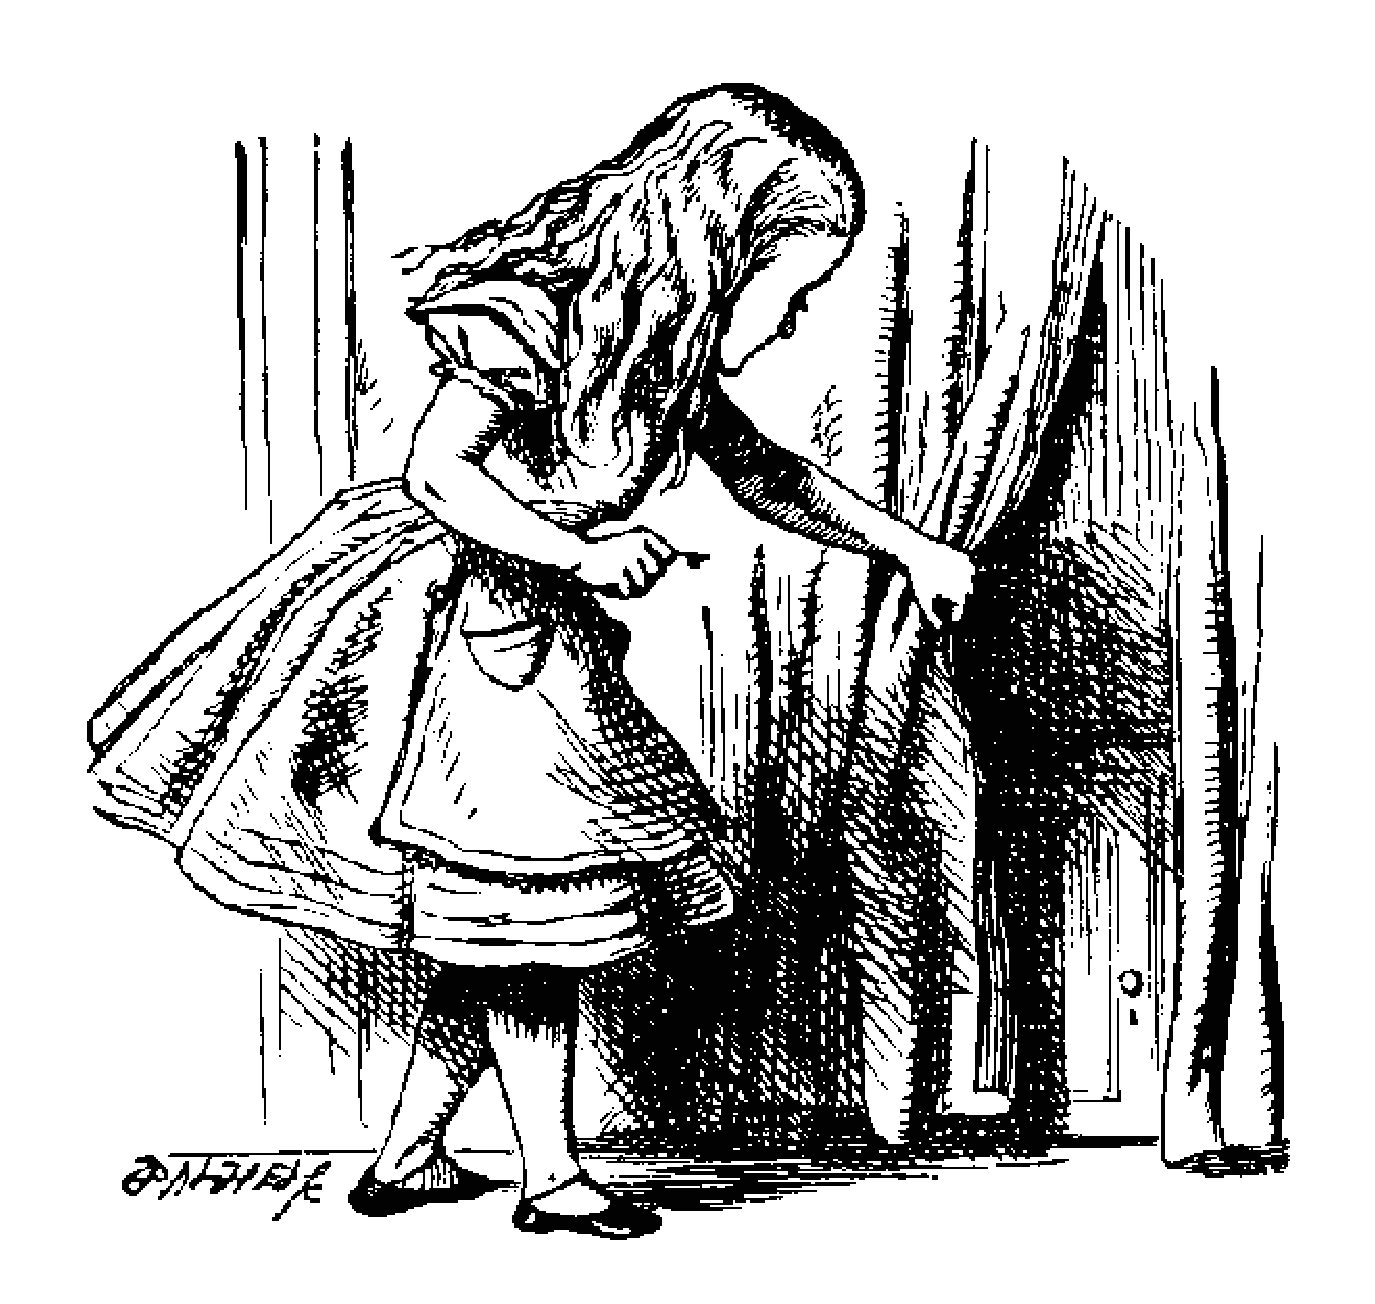
\includegraphics[width=7cm]{figures/alice}
\end{center}
\caption{Behind it was a little door}
\label{fig:alice}
\end{figure}

Alice opened the door (see Figure \ref{fig:alice}) and found that it
led into a small passage, not much larger than a rat-hole: she knelt
down and looked along the passage into the loveliest garden you ever
saw. How she longed to get out of that dark hall, and wander about
among those beds of bright flowers and those cool fountains, but she
could not even get her head through the doorway; ``and even if my head
would go through,'' thought poor Alice, ``it would be of very little
use without my shoulders. Oh, how I wish I could shut up like a
telescope! I think I could, if I only knew how to begin.'' For, you
see, so many out-of-the- way things had happened lately, that Alice
had begun to think that very few things indeed were really impossible.

%==============================================================================

\section{Choice of Colours}
\label{design}

The following diagrams (especially figure \ref{fig:alice}) illustrate the
process...

%==============================================================================
\section{Managing Dress Sense}
\label{managing}

In this chapter, we describe how the implemented the system.

%------------------------------------------------------------------------------
\section{Kangaroo Practices}



% - - - - - - - - - - - - - - - - - - - - - - - - - - - - - - - - - - - - - - -
\section{Knots and Bundles}
\label{sec:managing}


%------------------------------------------------------------------------------
\section{Conclusions}

Explain the wider lessons that you learned about software engineering,
based on the specific issues discussed in previous sections.  Reflect
on the extent to which these lessons could be generalised to other
types of software project.  Relate the wider lessons to others
reported in case studies in the software engineering literature.

%==============================================================================
\bibliographystyle{plain}
\bibliography{dissertation}
\end{document}
